\section{Braided Operads}

\begin{frame}{}
    \tableofcontents[currentsection]
\end{frame}

\begin{frame}{Braided Operads}
      \begin{defin}
        An {\em operad} $\B$ in $\C$ consists of 
        \begin{itemize}
        \item a family of objects $(\B(j))_{j \in \N}$
        \item a unit morphism $\eta \colon k \rightarrow \B(1)$
        \item a composition morphism
        \[
            \gamma \colon \B(k) \otimes \B(j_1) \otimes \cdots \otimes \B(j_k) \rightarrow \B(j),
        \]
        where $\sum_{1 \leq i \leq k} j_i = j$ 
        \item an action of $B_n$ on $\B(n)$ 
        \end{itemize}
        such that suitable associativity, equivariance, unitality constraints
        hold.
      \end{defin}
\end{frame}

\begin{frame}[fragile]{Example: Braid Operad}
Let $\B$ be the {\em braid operad} defined by $\B(n) \coloneqq B_n$, where $B_n$
            denotes the braid group on $n$ strands. The composition morphism 
        \[
            \gamma \colon B_k \times B_{j_1} \times \dots \times B_{j_k} \to B_{j}, \;
            (\tau, (\sigma_i)_{1 \leq i \leq k}) \mapsto \tau(\sigma_1 \oplus \dots \oplus \sigma_k),
        \]

        where $\tau(\sigma_1 \oplus \dots \oplus \sigma_k)$ denotes the braid
        that $\tau$-braids $k$ many blocks.
    \begin{center}
        $\vcenter{\hbox{\begin{tikzpicture}[ braid/.cd, strand 1/.style={black,
            line width=1.5pt}, strand 2/.style={black, line width=1.5pt}, strand
            3/.style={blue, line width=1.5pt}, strand 4/.style={magenta, line
            width=1.5pt}, strand 5/.style={red, line width=1.5pt}, strand
            6/.style={amber, line width=1.5pt}, ] \pic at (0,0)
            {braid={s_1-s_3-s_5}}; \end{tikzpicture}}}$
        \quad
        $\rightsquigarrow$
        \quad
        $\vcenter{\hbox{\begin{tikzpicture}[ braid/.cd, strand 1/.style={blue,
            line width=1.5pt}, strand 2/.style={magenta, line width=1.5pt},
            strand 3/.style={red, line width=1.5pt}, strand 4/.style={amber,
            line width=1.5pt}, ] \pic at (0,0) {braid={s_1-s_3 s_{1,2,3}
            s_{2,3,4}}}; \end{tikzpicture}}}$
    \end{center}
    The associativity and unitality conditions follow from the group conditions.
\end{frame}

% \begin{frame}
    % \begin{itemize}
    %     \item Another example is the universal cover operad of $\E_2$. Consider
    %     the unordered little disk space $\E_2 \slash S$. By Fox and Neuwirth
    %     (c.f. \cite{fox}): the fundamental group of $\E_2(n) \slash S_n$ is the
    %     $n$-th braid group $B_n$.

        % \begin{rem}
        %     For a finite set $I$, we consider the little disks in $\E_2(n)$ as
        %     labeled by $I$ instead of $\{1,...,n\}$, called $I$-labeled
        %     configuration.
        % \end{rem} 
 

% \end{frme}

\begin{frame}[fragile]
    \begin{defin}
    \small{The $\Grp$-enriched category $\Br$ of {\em braided sets}:
    \begin{enumerate}[(i)]
        \item Objects are finite sets.
        \item A morphism $\widetilde{\alpha} \colon I \to J$ in $\Br$ consists
        of 
        \begin{itemize}
            \item a map of finite sets  $\alpha \colon I \to J$
            \item For all $j \in J$ $\alpha_j$-labeled configuration
        $\left\{\widetilde{\alpha_j} \right\}$.
    
        \end{itemize}
        \item Composition: consists of composing maps of finite sets and
        "inserting disks", analogously to the composition in the little disk
        operad $\E_2$.

        
        % analogously to the composition map in $\Ex$ as defined above.
        \item Identity morphism $\id_I$ is given by the identity configurations
        $\id^{(i)}$.

        \item For morphisms $\widetilde{\alpha}, \widetilde{\beta} \colon I \to
        J$ in $\Br$ with $\alpha = \beta$, a
        $2$-morphism in $\Br$ consists of a family of homotopy classes of paths,
        $ j \in J$:
        $$
            \eta_j \colon \widetilde{\alpha_j} \Rightarrow \widetilde{\beta_j}.
        $$
    \end{enumerate}}
\end{defin}
\end{frame}

\begin{frame}[fragile]
\tiny{\begin{defin}A {\em colored braided operad} $\B$ consists of the following
    data:
    \begin{enumerate}[(i)]
        \item A collection $\{X,Y,Z, \dots\}$ of colors.
        \item For $I$-labeled configuration $\widetilde{I}$,
         collection of
        colors $\{X_i\}_{i \in I}$, color $Y$, 
        a set of
        morphisms:
        $\Mul_{\B}^{\widetilde{I}}(\{X_i\}_{i \in I}, Y)$.
        \item For every triangle in $\Br$:
        \begin{center}
            \begin{adjustbox}{max height = 2cm}
            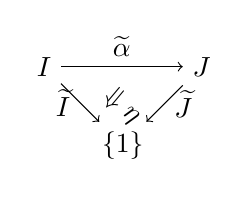
\begin{tikzpicture}
                % Define node positions
                \node (B) at (0, 1) {$I$}; \node (C) at (2, 1) {$J$}; \node (A)
                at (1, 0) {$\{ 1 \}$};
                
                % Draw arrows
                \draw[->] (B) -- (C) node[midway, above] { $\widetilde{\alpha}$};
                \draw[->] (B) -- (A) node[midway, left] { $\widetilde{I}$};
                \draw[->] (C) -- (A) node[midway, right] {$\widetilde{J}$};
                
                % Natural transformation arrow
                \node[rotate=-40] at (1, 0.5) {$\Downarrow \eta$};
                % \node at (1.7, 1.2) {$\eta$};
            \end{tikzpicture}
        \end{adjustbox}
        \end{center}
        % along with collections of colors $\{X_i\}_{i \in I}$, $\{Y_j\}_{j \in
        % J}$ and color $Z$, 
        a composition map:
        \[
            \gamma \colon \prod_{j \in J} \Mul_{\B}^{\widetilde{\alpha_j}}\left(\{X_i\}_{i \in \alpha_j}, Y_j\right) \times \Mul_{\B}^{\widetilde{J}}\left(\{Y_j\}_{j\in J}, Z\right) \to \Mul_{\B}^{\widetilde{I}}\left(\{X_i\}_{i \in I}, Z\right).  
        \]
        \item For any $I$-labeled configuration $\widetilde{I}$, $|I|=1$, color
        $X$, an identity morphism: $\id_X \in
        \Mul_{\B}^{\widetilde{I}}(\{X\}, X)$
        \end{enumerate}
        The data satisfies associativity and unitality constraints. \end{defin}}
\end{frame}

\begin{frame}
    \begin{prop}
        A unicolored braided operad defines a braided operad.
    \end{prop}
        We set:
        \[
            \B(n) \coloneqq \Mul^{b_n}(\{X\}^n, X)
        \]
        for the configuration $b_n$:
\begin{center}
        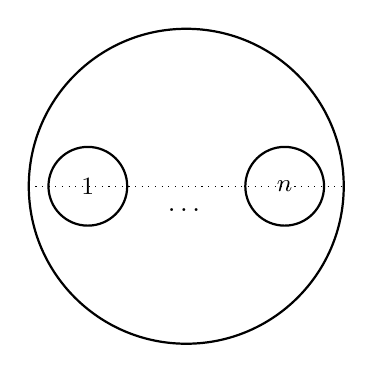
\begin{tikzpicture}
        %basepoint
        \draw[thick] (1,0) circle (2); \draw[thick] (2.25, 0) circle (0.5);
        \draw[thick] (-0.25, 0) circle (0.5);
        \node at (-0.25, 0) {\small $1$};
        \node at (1, -0.3) {\dots};
        \node at (2.25, 0) {\small $n$};
        \draw[dotted](-1, 0)--(3, 0);
    \end{tikzpicture}
\end{center}
\end{frame}

\begin{frame}
\small{\begin{defin}
    The category of braided pointed sets, $\Brr$, is the following
    $\Grp$-enriched category:
    \begin{enumerate}[(i)]
        \item The objects of $\Brr$ are finite sets with a distinguished point
        $\ast$.
        \item A morphism $\widetilde{\alpha}_{\ast} \colon I \to J$ consists of
        a ma $\alpha \colon I \to J$ with $\alpha(\ast)=\ast$ together with a
        morphism in $\Br$:
        \[
            \widetilde{\alpha} \colon \alpha^{-1}(J \setminus \{\ast\}) \to J \setminus \{\ast\}
        \]
        
        \item For morphisms $\widetilde{\alpha}_{\ast}, \widetilde{\beta}_{\ast}
        \colon I \to J$ with the same underlying map $\alpha = \beta$, a
        $2$-morphism $\eta_{\ast} \colon \widetilde{\alpha}_{\ast} \to
        \widetilde{\beta}_{\ast}$ corresponds to a $2$-morphism $\eta \colon
        \widetilde{\alpha} \Rightarrow \widetilde{\beta}$ in $\Br$.
    \end{enumerate}
\end{defin}

\begin{defin}
    Let the category of standard braided pointed sets $\Brx$ be the full
    subcategory of $\Brr$ on the objects $\langle n \rangle$, $n \in \N$.
    \end{defin}}
\end{frame}

\begin{frame}
    \small{\begin{defin} Let $\B$ be a colored braided operad. Define the
    $\Grp$-enriched category $\Bx$:
    \begin{enumerate}[(i)]
        \item Objects are finite sequences $\{X_i\}_{1 \leq i \leq n}$ of colors
        of $\B$.
        \item For objects $\{X_i\}_{1 \leq i \leq m}$, $\{Y_j\}_{1 \leq j \leq
        n}$, a morphism 
        \[
            \phi \colon \{X_i\}_{1 \leq i \leq m} \to \{Y_j\}_{1 \leq j \leq n}
        \]
        given by $\widetilde{\alpha} \colon \langle m \rangle \to \langle n
        \rangle$ in $\Brx$ together with for $1 \leq j \leq n$:
        \[
            \phi_j \in \Mul_{\B}^{\widetilde{\alpha_j}}(\{X_i\}_{i \in \alpha^{-1}(j)}, Y_j)
        \]
        in $\B$. We call $\widetilde{\alpha}$ the underlying morphism of $\phi$.
        \item Composition of morphisms is determined by the composition in
        $\Brx$ and $\B$.
        \item For morphisms $\phi, \psi$, a $2$-morphism $\bar{\eta} \colon \phi
        \to \psi$ consist of a $2$-morphism 
        $$\widetilde{\eta} \colon \widetilde{\alpha_{\phi}} \Rightarrow
        \widetilde{\alpha_{\psi}}$$ in $\Brx$ such that $\gamma((\id_{X_i})_{i
        \in \alpha_{\phi_j}}, \psi_j) = \phi_j$ for $\gamma$ corresponding to
        $\widetilde{\eta_j}$.
    \end{enumerate}
\end{defin}}
\end{frame}

\begin{frame}
Let $\B$ be a colored braided operad. There is a forgetful functor 
\[
\pi \colon \Bx \to \Brx
\]
\pause
\begin{thm}
For $\pi$ satisfies the following properties:
    \begin{enumerate}[(M1)]
        \item \textbf{Op-fibration condition:} $\pi$ is a Grothendieck
        op-fibration. 
        \item \textbf{Segal condition:} $\C \cong \Bx_{\langle 1 \rangle}$ and
        $\Bx_{\langle n \rangle} \cong \C^n$.
    \end{enumerate}
We can construct a braided monoidal structure on $\C$.
\end{thm}

We suspect the construction is reversible, i.e. we can construct a colored braided operad from a braided monoidal category.
\end{frame}

\begin{frame}[fragile]
    We define $\otimes \colon \C^2 \to \C$, by lifting the following morphism in
    $\Brx$:
   \begin{align*}
    \mu \colon \langle 2 \rangle &\to \langle 1 \rangle \\
    1 &\mapsto 1 \\
    2 &\mapsto 1 \\
\end{align*}
with configuration $b_2 \in \E_2(2)$:
\begin{center}
    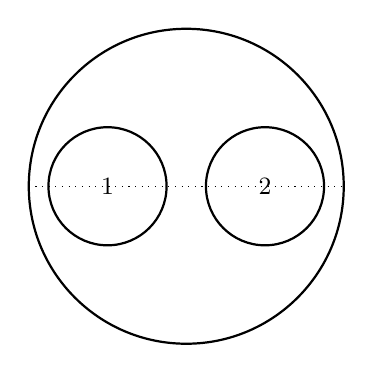
\begin{tikzpicture}
                        % First element (left)
                        \node at (1, 0) {\small $2$}; \node at (-1, 0) {\small
                        $1$};
                        
                        \draw[thick] (0,0) circle (2); \draw[thick] (1, 0)
                        circle (0.75); \draw[thick] (-1, 0) circle (0.75);
                        \draw[dotted](-2, 0)--(2, 0);       
        \end{tikzpicture}
\end{center}
\end{frame}




\begin{frame}[fragile]
    \small{Let $\beta \colon \langle 2 \rangle \to \langle 2 \rangle$ with
    $\beta(1)=2$, $\beta(2)=1$ denote the morphism in $\Brx$ with the trivial
    configurations $(\id^{2}, \id^{1})$.

    We need to choose a homotopy class of paths for: \adjustbox{max height =
    2cm}{
    \begin{tikzcd}
        \langle 2 \rangle \arrow[r, "\beta"] \arrow[d, "\mu"] & \langle 2
        \rangle \arrow[d, "\mu"] \\
        \langle 1 \rangle  \arrow[r, dashed]                  & \langle 1
        \rangle                
    \end{tikzcd}}

    We choose the half twist: \adjustbox{max height = 3cm, right}{
    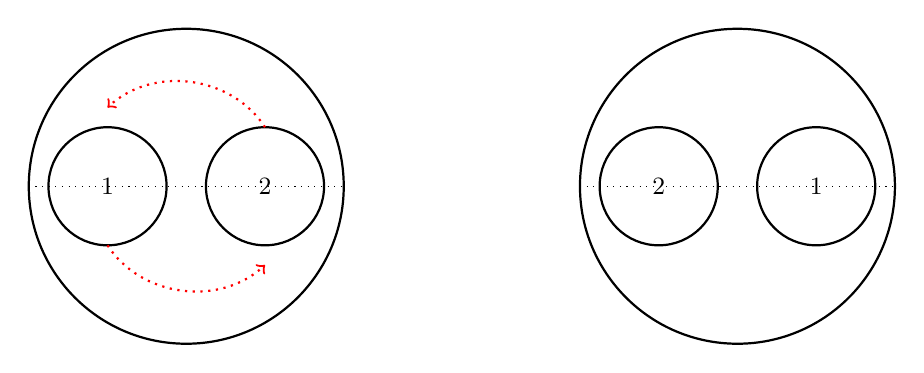
\begin{tikzpicture}
                        % basepoint
                        \node at (1, 0) {\small $2$}; \node at (-1, 0) {\small
                        $1$};
                         
                        \draw[thick] (0,0) circle (2); \draw[thick] (1, 0)
                        circle (0.75); \draw[thick] (-1, 0) circle (0.75);
                        \draw[dotted](-2, 0)--(2, 0); \draw[->, thick, dotted,
                        red] (-1, -0.75) to [bend right=50] (1, -1); \draw[->,
                        thick, dotted, red] (1, 0.75) to [bend right=50] (-1,
                        1);

                        \node at (3.5, 0) {$\rightsquigarrow$};
                        
                        % twisted basepoint
                        \node at (8, 0) {\small $1$}; \node at (6, 0) {\small
                        $2$};
                        
                        \draw[thick] (7,0) circle (2); \draw[thick] (8, 0)
                        circle (0.75); \draw[thick] (6, 0) circle (0.75);
                        \draw[dotted](5, 0)--(9, 0);      
        \end{tikzpicture}}}
Similarly, we define the associator. Thus, we obtain in fact a braided monoidal structure on $\C$.
\end{frame}

% \begin{frame}[fragile]
%     Similarly, for the associator, we choose a path along the horizontal line:

%     \medskip

%     \begin{tikzpicture}
%         % First element (left)
%         \node at (-1, 0) {\small $1$}; \node at (0.625, 0) {\small $2$}; \node
%         at (1.375, 0) {\small $3$}; \draw[thick] (0,0) circle (2); \draw[thick]
%         (-1, 0) circle (0.75); \draw[thick] (0.625, 0) circle (0.275);
%         \draw[thick] (1.375, 0) circle (0.275); \draw[dotted] (1, 0) circle
%         (0.75); \draw[dotted](-2, 0)--(2, 0);

%         \node at (3.5, 0) {$\overset{\eta}{\rightsquigarrow}$};

%         % Second element (left)
%         \node at (5.625, 0) {\small  $1$}; \node at (6.375, 0) {\small $2$};
%         \node at (8, 0) {\small$3$}; \draw[thick] (7,0) circle (2);
%         \draw[dotted] (6, 0) circle (0.75); \draw[thick] (6.325, 0) circle
%         (0.275); \draw[thick] (5.675, 0) circle (0.275); \draw[thick] (8, 0)
%         circle (0.75); \draw[dotted](5, 0)--(9, 0);     
%     \end{tikzpicture}
    
%     \medskip

% This defines in fact a braided monoidal structure on $\C$.
% \end{frame}

% \begin{frame}[fragile] \begin{table} $$\otimes \colon \C^2 \to \C$$ &
%     $\begin{aligned} \mu \colon \langle 2 \rangle &\to \langle 1 \rangle \\
%     1 &\mapsto 1 \\
%     2 &\mapsto 1 \\
%     \end{aligned}$ & \begin{adjustbox}{max height = 2cm} \begin{tikzpicture} %
%     basepoint \node at (1, 0) {\small $2$}; \node at (-1, 0) {\small $1$};
                        
%                         \draw[thick] (0,0) circle (2); \draw[thick] (1, 0)
%                         circle (0.75); \draw[thick] (-1, 0) circle (0.75);
%                         \draw[dotted](-2, 0)--(2, 0); \draw[->, thick, dotted,
%                         red] (-1, -0.75) to [bend right=50] (1, -1); \draw[->,
%                         thick, dotted, red] (1, 0.75) to [bend right=50] (-1,
%                         1);

%                         \node at (2.75, 0) {$\rightsquigarrow$};
                        
%                         % twisted basepoint \node at (6.5, 0) {\small $1$};
%                         \node at (4.5, 0) {\small $2$};
                        
%                     \draw[thick] (5.5,0) circle (2); 
%                     \draw[thick] (6.5, 0) circle (0.75); 
%                     \draw[thick] (4.5, 0) circle (0.75);
%                     \draw[dotted](3.5, 0)--(7.5, 0);
%         \end{tikzpicture}
%     \end{adjustbox} \\
%     x & n & \begin{adjustbox}{max height = 2cm} \begin{tikzpicture} % First
%     element (left) \node at (1, 0) {\small $2$}; \node at (-1, 0) {\small
%     $1$};
                        
%                         \draw[thick] (0,0) circle (2); \draw[thick] (1, 0)
%                         circle (0.75); \draw[thick] (-1, 0) circle (0.75);
%                         \draw[dotted](-2, 0)--(2, 0);       
%         \end{tikzpicture}
%     \end{adjustbox}
%     \end{table}
% \end{frame}

% \begin{frame}[fragile]{Version with Better Control} \begin{table} \centering %
%     \renewcommand{\arraystretch}{2} \begin{tabular}{ccc} \centering $\otimes
%     \colon \C^2 \to \C$ & \centering $\mu \colon \langle 2 \rangle
%     \overset{\text{active}}{\to} \langle 1 \rangle$ & \centering
%     \begin{adjustbox}{max height = 2cm} $\begin{tikzpicture} % basepoint \node
%     at (1, 0) {\small $2$}; \node at (-1, 0) {\small $1$}; \draw[thick] (0,0)
%     circle (2); \draw[thick] (1, 0) circle (0.75); \draw[thick] (-1, 0) circle
%     (0.75); \draw[dotted](-2, 0)--(2, 0); \draw[->, thick, dotted, red] (-1,
%     -0.75) to [bend right=50] (1, -1); \draw[->, thick, dotted, red] (1, 0.75)
%     to [bend right=50] (-1, 1); \node at (2.75, 0) {$\rightsquigarrow$}; %
%     twisted basepoint \node at (6.5, 0) {\small $1$}; \node at (4.5, 0)
%     {\small $2$}; \draw[thick] (5.5,0) circle (2); \draw[thick] (6.5, 0)
%     circle (0.75); \draw[thick] (4.5, 0) circle (0.75); \draw[dotted](3.5,
%     0)--(7.5, 0); \end{tikzpicture}$ \end{adjustbox} \\
%             \centering x & \centering n & \centering \begin{adjustbox}{max
%             height = 2cm} $\begin{tikzpicture} % First element (left) \node at
%             (1, 0) {\small $2$}; \node at (-1, 0) {\small $1$}; \draw[thick]
%             (0,0) circle (2); \draw[thick] (1, 0) circle (0.75); \draw[thick]
%             (-1, 0) circle (0.75); \draw[dotted](-2, 0)--(2, 0);
%             \end{tikzpicture}$ \end{adjustbox} \end{tabular} \end{table}
%             \end{frame}




% \begin{frame}{Properties of $\pi$ - (1/2)} \small{\begin{prop} Let $\B$ be a
%     colored braided operad. The forgetful functor
%     \[
%         \pi \colon \Bx \to \Brx
%     \]
%     has the following properties:
%     \begin{enumerate}
%         \item For every inert morphism $\widetilde{\alpha} \colon \langle n
%         \rangle \to \langle m \rangle$  in $\Brx$ and object $X \in \Bx$ there
%         exists a $\pi$-cocartesian morphism $f \colon X \to X'$ lifting
%         $\widetilde{\alpha}$ . In particular $\widetilde{\alpha}$ induces a
%         functor 
%         $$\pi_{\widetilde{\alpha}} \colon \Bx_{\langle n \rangle} \to
%         \Bx_{\langle m \rangle}.$$
%         \item For every pair of objects $X,Y$ in $\Bx$ the functor
%         \[
%                 \Hom_{\Bx}(X,Y) \to \Hom_{\Brx}(\pi(X),\pi(Y))
%         \]
%         is a fibration.
%         \item For a morphism $\widetilde{\alpha}$ in $\Brx$, the groupoid of
%         morphisms lying over $\widetilde{\alpha}$:
%         $$\Hom_{\D}^{\widetilde{\alpha}}(X, X')$$ is discrete.
%         \end{enumerate}
%         \vspace{0.2cm}
%         \textit{(continued on next slide...)}
%         \end{prop}}
% \end{frame}


% \begin{frame}{Properties of $\pi$ - (2/2)} \small{\begin{prop}[Properties of
%     $\pi$ (continued)] \begin{enumerate}[(i)] \setcounter{enumi}{3} \item Let
%     $X = [X_1, \dots, X_n] \in \Bx_{\langle n \rangle}$ and $X' = [X_1',
%     \dots, X_m'] \in \Bx_{\langle m \rangle}$ be objects, $\alpha : \langle n
%     \rangle \to \langle m \rangle$ be a morphism in $\Brx$ and let
%     $\Hom_{\Bx}^{\alpha}(X, X')$ be the set if morphisms over $\alpha$. Choose
%     $\pi$-cocartesian morphisms $X' \to X'_i$ lying over the inert morphism
%     $\rho^i \colon \langle n \rangle \to \langle 1 \rangle$ for $1 \leq i \leq
%     n$. Then the induced map
%         \[
%             \Hom_{\Bx}^{\alpha}(X, X') \to \prod_{1 \leq i \leq n} \Hom_{\Bx}^{\rho^i \circ \alpha}(X, X_i')
%         \]
%         is an equivalence of groupoids. 
        
%         \item For every finite collection of objects $X_1, \dots, X_n \in
%         \Bx_{\langle 1 \rangle}$, there exists an object $X \in \Bx_{\langle n
%         \rangle}$ and a collection of $p$-cocartesian morphism $X \to X_i$
%         covering $\rho^i \colon \langle n \rangle \to \langle 1 \rangle$.
%         % \item For all $n \in \N$, there is an equivalence of categories
%         % \[
%         %     \Bx_{\langle n \rangle} \cong \left(\Bx_{\langle 1 \rangle}\right)^n
%         % \]
%         % induced by the morphism $\rho^i$ from Example \ref{eg:rho_i}.
%     \end{enumerate}
% \end{prop}} \end{frame}

\begin{frame}{Operadic Fibration - Definition (1/2)}
    \small{\begin{defin}[Operadic Fibration]
        An {\em operadic fibration} is a functor between $\Grp$-enriched
        categories
        \[
        \pi \colon \D \to \Brx
        \]
        satisfying the following conditions:
        \begin{enumerate}[(i)]
            \item The functor $\pi$ is a categorical fibration.
            \item For every inert morphism $\widetilde{\alpha} \colon \langle n
            \rangle \to \langle m \rangle$ in $\Brx$ and object $X \in
            \mathcal{D}$ there exists a $\pi$-cocartesian morphism $f \colon X
            \to X'$ lifting $\widetilde{\alpha}$.
            \item For a morphism $\widetilde{\alpha}$ in $\Brx$,
            the groupoid of morphisms lying over $\widetilde{\alpha}$:
            $$\mathrm{Hom}_{\mathcal{D}}^{\widetilde{\alpha}}(X, X')$$ is
            discrete.
        \end{enumerate}
        \vspace{0.2cm}
        \textit{(continued on next slide...)}
    \end{defin}}
\end{frame}

\begin{frame}{Operadic Fibration - Definition (2/2)}
    \small{\begin{defin}[Operadic Fibration (continued)]
        \begin{enumerate}[(i)]
            \setcounter{enumi}{3}
            \item Let $X \in \mathcal{D}_{\langle n \rangle}$ and $X' \in
            \mathcal{D}_{\langle m \rangle}$ be objects, $\widetilde{\alpha} :
            \langle n \rangle \to \langle m \rangle$ be a morphism in
            $\Brx$ and let 
            $$\mathrm{Hom}_{\mathcal{D}}^{\widetilde{\alpha}}(X, X')$$ be the
            morphisms which lie over $\widetilde{\alpha}$. Choose
            $\pi$-cocartesian morphisms $X' \to X'_i$ lying over the inert
            morphism $\rho^i \colon \langle n \rangle \to \langle 1 \rangle$ for
            $1 \leq i \leq n$. Then the induced map
            \[
            \mathrm{Hom}_{\mathcal{D}}^{\widetilde{\alpha}}(X, X') \to \prod_{1 \leq i \leq n} \mathrm{Hom}_{\mathcal{D}}^{\rho^i \circ \widetilde{\alpha}}(X, X_i')
            \]
            is an equivalence of groupoids.
            \item For every finite collection of objects $X_1, \dots, X_n \in
            \D_{\langle 1 \rangle}$, there is an object $X \in \D_{\langle n
            \rangle}$ and a collection of $\pi$-cocartesian morphism $X \to X_i$
            covering $\rho^i \colon \langle n \rangle \to \langle 1 \rangle$.
        \end{enumerate}
    \end{defin}}
\end{frame}

\begin{frame}[fragile]
    \begin{prop}
    Let $\B$ be a colored braided operad and $\pi$ the forgetful functor
    
    \vspace{0.3cm}

    $\begin{aligned} \pi \colon \Bx &\to \Brx \\
        [X_1, \dots, X_n] &\mapsto \langle n \rangle \\
        (f \colon [X_1, \dots, X_n] \to [X_1', \dots, X_m']) &\mapsto (\alpha_f
        \colon \langle n \rangle \to \langle m \rangle) \\
        (\eta \colon \psi \Rightarrow \phi) &\mapsto (\widetilde{\eta} \colon
    \alpha_{\phi} \Rightarrow \alpha_{\psi}) \end{aligned}$

    \vspace{0.5cm}

    where $\alpha_f$ refers to the morphism in $\Brx$ underlying $f$ and
    $\widetilde{\eta}$ the $2$-morphism underlying $\eta$. 
    \vspace{0.5cm}

    Then, $\pi$ is an operadic fibration.
\end{prop}
\end{frame}


\begin{frame}
    \begin{prop}
    Let
    \[
        \pi \colon \D \to \Brx
    \]
    be an operadic fibration over $\Brx$. Then we can reconstruct a colored
    braided operad $\B$ from $\D$ such that, $\D \cong \Bx$ and the functor
    \[
        \Bx \cong \D \overset{\pi}{\to} \Brx
    \]
    is the usual forgetful functor from $\Bx$ to $\Brx$.
\end{prop}
\end{frame}

\begin{frame}{Outlook}
    Next possible steps:
    \begin{itemize}
        \item Drop the condition that $$\mathrm{Hom}_{\mathcal{D}}^{\widetilde{\alpha}}(X, X')$$ is
            discrete. We suspect this gives a notion that is equivalent to colored braided operads in $\Grp$.
        \item Further generalization to $\infty$-categories gives a notion that is equivalent to colored braided operads in $\Top$.
        \item Consider examples of colored braided operads and their algebras.
    \end{itemize}
\end{frame}